\section{Spatial Discretization Schemes}
\label{spatialdiscretization}

We discretize space with the cell-centered finite volume method (\ref{cc} ), the box method (\ref{box})
or a staggered grid scheme.
Grid adaption is available for both box and cell-centered finite volume method.
In general, the spatial  parameters, especially the porosity, have to be assigned on
the coarsest level of discretization.

\subsection{Box Method -- A Short Introduction}\label{box}

The so called box method unites the advantages of the finite-volume (FV) and
finite-element (FE) methods.

First, the model domain $\Omega$ is discretized with a FE mesh consisting of nodes
$i$ and corresponding elements $E_k$. Then, a secondary FV mesh is constructed
by connecting the midpoints and barycenters of the elements surrounding node
$i$ creating a box $B_i$ around node $i$ (see Figure \ref{pc:box}a).

\begin{figure} [ht]
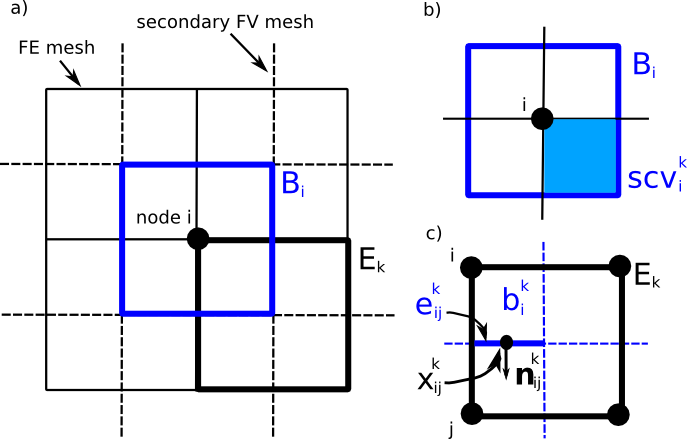
\includegraphics[width=0.8\linewidth,keepaspectratio]{png/box_disc.png}
\caption{\label{pc:box} Discretization of the box method}
\end{figure}

The FE mesh divides the box $B_i$ into subcontrolvolumes (scv's) $b^k_i$
(see Figure \ref{pc:box}b). Figure \ref{pc:box}c shows the finite element $E_k$
and the scv's $b^k_i$ inside $E_k$, which belong to four different boxes $B_i$.
Also necessary for the discretization are the faces of the subcontrolvolumes (scvf's)
$e^k_{ij}$ between the scv's $b^k_i$ and $b^k_j$, where $|e^k_{ij}|$ is the length
of the scvf. The integration points $x^k_{ij}$ on $e^k_{ij}$ and the outer normal
vector $\mathbf n^k_{ij}$ are also to be defined (see Figure \ref{pc:box}c).

The advantage of the FE method is that unstructured grids can be used, while the
FV method is mass conservative. The idea is to apply the FV method (balance of
fluxes across the interfaces) to each FV box $B_i$  and to get the fluxes across
the interfaces $e^k_{ij}$ at the integration points $x^k_{ij}$ from the FE approach.
Consequently, at each scvf the following expression results:

\begin{equation}
 	f(\tilde u(x^k_{ij})) \cdot \mathbf n^k_{ij} \: |e^k_{ij}| \qquad \textrm{with}
 	\qquad \tilde u(x^k_{ij}) = \sum_i N_i(x^k_{ij}) \cdot \hat u_i .
\end{equation}

In the following, the discretization of the balance equation is going to be derived.
From the \textsc{Reynolds} transport theorem follows the general balance equation:

\begin{equation}
	\underbrace{\int_\Omega \frac{\partial}{\partial t} \: u \: dx}_{1}
	+ \underbrace{\int_{\partial\Omega} (\mathbf{v} u + \mathbf w) \cdot \textbf n \: d\varGamma}_{2} = \underbrace{\int_\Omega q \: dx}_{3}
\end{equation}

\begin{equation}
	f(u) = \int_\Omega \frac{\partial u}{\partial t} \: dx + \int_{\Omega} \nabla \cdot
	\underbrace{\left[  \mathbf{v} u + \mathbf w(u)\right] }_{F(u)}  \: dx - \int_\Omega q \: dx = 0
\end{equation}
where term 1 describes the changes of entity $u$ within a control volume over
time, term 2 the advective, diffusive and dispersive fluxes over the interfaces
of the control volume and term 3 is the source and sink term. $\Omega$ denotes the
model domain and $F(u) = F(\mathbf v, p) = F(\mathbf v(x,t), p(x,t))$.

Like the FE method, the box method follows the principle of weighted residuals.
In the function $f(u)$ the unknown $u$ is approximated by discrete values at the
nodes of the FE mesh $\hat u_i$ and linear basis functions $N_i$ yielding an
approximate function $f(\tilde u)$. For $u\in \lbrace \mathbf v, p, x^\kappa \rbrace$
this means:

\begin{minipage}[b]{0.47\textwidth}
\begin{equation}
\label{eq:p}
	\tilde p = \sum_i N_i \hat{p}_i
\end{equation}
\begin{equation}
\label{eq:v}
	\tilde{\mathbf v} = \sum_i N_i \hat{\mathbf v}_i
\end{equation}
\begin{equation}
\label{eq:x}
	\tilde x^\kappa  = \sum_i N_i \hat x_i^\kappa
\end{equation}
\end{minipage}
\hfill
\begin{minipage}[b]{0.47\textwidth}
\begin{equation}
\label{eq:dp}
	\nabla \tilde p = \sum_i \nabla N_i \hat{p}_i
\end{equation}
\begin{equation}
\label{eq:dv}
	\nabla \tilde{\mathbf v} = \sum_i \nabla N_i \hat{\mathbf v}_i
\end{equation}
\begin{equation}
\label{eq:dx}
	\nabla \tilde x^\kappa  = \sum_i \nabla N_i \hat x_i^\kappa .
\end{equation}
\end{minipage}

Due to the approximation with node values and basis functions the differential
equations are not exactly fulfilled anymore but a residual $\varepsilon$ is produced.

\begin{equation}
	f(u) = 0  \qquad \Rightarrow \qquad f(\tilde u) = \varepsilon
\end{equation}

Application of the principle of weighted residuals, meaning the multiplication
of the residual $\varepsilon$ with a weighting function $W_j$  and claiming that
this product has to vanish within the whole domain,

\begin{equation}
	\int_\Omega W_j \cdot \varepsilon \: \overset {!}{=} \: 0 \qquad \textrm{with} \qquad \sum_j W_j =1
\end{equation}
yields the following equation:

\begin{equation}
	\int_\Omega W_j \frac{\partial \tilde u}{\partial t} \: dx + \int_\Omega W_j
	\cdot \left[ \nabla \cdot F(\tilde u) \right]  \: dx - \int_\Omega W_j
	\cdot q \: dx = \int_\Omega W_j \cdot \varepsilon \: dx \: \overset {!}{=} \: 0.	
\label{eq:weightedResidual}	
\end{equation}

For standard Galerkin schemes, the weighting functions $W_j$ are chosen the same as the ansatz functions $N_j$. However, this does not yield a locally mass-conservative scheme. 
Therefore, for the Box method, the weighting functions $W_j$ are chosen as 
the piecewise constant functions over a
control volume box $B_j$, i.e.

\begin{equation}
	W_j(x) = \begin{cases}
	          1 &x \in B_j \\
		  0 &x \notin B_j.\\
	         \end{cases}
\label{eq:weightingFunctions}	         
\end{equation}
Thus, the Box method is a Petrov-Galerkin scheme, where the weighting functions do not belong to the same function space than the ansatz functions.

Inserting definition \eqref{eq:weightingFunctions} into equation \eqref{eq:weightedResidual} and using the \textsc{Green-Gaussian} integral theorem results in
\begin{equation}
	\int_{B_j} \frac{\partial \tilde u}{\partial t} \: dx + \int_{\partial B_j}  F(\tilde u) \cdot \mathbf n \: d\varGamma_{B_j} - \int_{B_j} q \: dx  \overset {!}{=} \: 0, 	
\label{eq:BoxMassBlance}	
\end{equation}
which has to hold for every box $B_j$. 

The first term in equation \eqref{eq:BoxMassBlance} can be written as
\begin{equation}
\int_{B_j} \frac{\partial \tilde u}{\partial t} \: dx = \frac{d}{dt} \int_{B_j} \sum_i \hat u_i N_i  \: dx = \sum_i \frac{\partial \hat u_i}{\partial t} \int_{B_j}  N_i  \: dx.
\end{equation} 
Here, a mass lumping technique is applied by assuming that the storage capacity is
reduced to the nodes. This means that the integrals $M_{i,j} = \int_{B_j}  N_i \: dx$
are replaced by some mass lumped terms $M^{lump}_{i,j}$ which are defined as
\begin{equation}
	 M^{lump}_{i,j} =\begin{cases}  V_j &j = i\\
	0 &j \neq i,\\
	         \end{cases}
\end{equation}
where $V_j$ is the volume of the FV box $B_j$ associated with node $j$.
The application of this assumption yields

\begin{equation}
\label{eq:disc1}
	V_j \frac{\partial \hat u_j}{\partial t}
	+  \int_{\partial B_j}  F(\tilde u) \cdot \mathbf n \: d\varGamma_{B_j} - Q_j = 0,
\end{equation}
where $Q_j$ is an approximation (using some quadrature rule) of the integrated source/sink term $\int_{B_j} q \: dx$.

Using an implicit Euler time discretization finally
leads to the discretized form which will be applied to the mathematical
flow and transport equations:

\begin{equation}
\label{eq:discfin}
	V_j \frac{\hat u_j^{n+1} - \hat u_j^{n}}{\Delta t}
	+ \int_{\partial B_j}  F(\tilde u^{n+1}) \cdot \mathbf n
	\;  d{\varGamma}_{B_j} - Q_j^{n+1} \: = 0.
\end{equation}
Equation \eqref{eq:discfin} has to be fulfilled for each box $B_j$.

\subsection{Cell Centered Finite Volume Methods -- A Short Introduction}\label{cc}

\begin{figure} [ht]
\centering
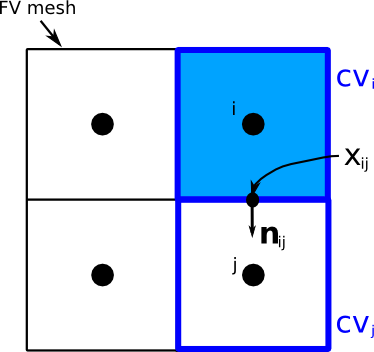
\includegraphics[width=0.4\linewidth,keepaspectratio]{png/cc_disc.png}
\caption{\label{pc:cc} Discretization of the cell centered finite volume method}
\end{figure}

The cell-centered finite volume method uses the elements of the grid as control volumes.
For each control volume all discrete values are determined at the element/control
volume center (see Figure~\ref{pc:cc}).
The mass or energy fluxes are evaluated at the integration points ($x_{ij}$),
which are located at the midpoints of the control
volume faces. This is a two point flux approximation since the flux between
the element/control volume centers $i$ and $j$ is calculated
only with information from these two points. In contrast the box method uses
a multi-point flux approximation where all nodes of the
element influence the flux between two specific nodes. \par
Neumann boundary conditions are applied at the boundary control volume faces
and Dirichlet boundary conditions at the boundary control volumes. \par
The cell centered finite volume method is robust and mass conservative but
should only be applied for structured grids
(the control volume face normal vector ($n_{ij}$) should be parallel to the
direction of the gradient between the two element/control
volume centers).

We consider a domain $\Omega \in \mathbb{R}^d$, $d \in \{ 2, 3 \}$ with boundary $\Gamma = \bar{\Omega} / \Omega$ and the following elliptic model problem:

\begin{equation}
  \begin{aligned}
                   \nabla \cdot \left( - \mathbf{\Lambda} \nabla u \right) &= q   &&\mathrm{in} \, \Omega \\
               \left( - \mathbf{\Lambda} \nabla u \right) \cdot \mathbf{n} &= v_N &&\mathrm{on} \, \Gamma_N \\
                                                                   u &= u_D &&\mathrm{on} \, \Gamma_D.
    \label{eq:elliptic}
  \end{aligned}
\end{equation}

Here, $\mathbf{\Lambda} = \mathbf{\Lambda}(\mathbf{x}, \mathbf{u})$ is a symmetric and positive definite tensor of second rank, $u = u (\mathbf{x})$ is unknown and $q = q(\mathbf{x}, \mathbf{u})$ is a source/sink. For the derivation of the finite-volume formulation we integrate the first equation of \eqref{eq:elliptic} over $\Omega$ and apply the Gauss divergence theorem:

\begin{equation}
    \int_{\Gamma} \left( - \mathbf{\Lambda} \nabla u \right) \cdot \mathbf{n} \mathrm{d} \Gamma = \int_\Omega q \mathrm{d}\Omega.
    \label{eq:ellipticIntegrated}
\end{equation}

We denote by $\mathcal{M}$ the mesh that results from the division of the domain $\Omega$ into $n_e$ control volumes $K_i$. Each $K_i$ is a polygonal open set and $\mathring{K_i} \mathring{\cap K_j} = \emptyset, \forall{i \neq j}$ and $\Omega = \cup_i^{n_e} K_i$. We then enforce equation \eqref{eq:ellipticIntegrated} to be fulfilled in each control volume, which leads to

\begin{equation}
    \sum_{\sigma \in K} F_{K, \sigma} = Q_K, \forall_{K \in \mathcal{M}}
\end{equation}

where $F_{K, \sigma} \approx \int_{\sigma} \left( - \mathbf{\Lambda} \nabla u \right) \cdot \mathbf{n} \mathrm{d} \Gamma$ is the discrete flux through a face $\sigma$ of cell $K$ and $Q_k = \int_K q \mathrm{d}x$ is the integrated source/sink term. 

\subsubsection{TPFA}\label{cc_tpfa}

 

\subsubsection{MPFA}\label{cc_mpfa}
Expressions for the face fluxes $F_{K, \sigma}$ are usually obtained by introducing intermediate face unknowns $\bar{u}_\sigma$ in addition to the cell unknowns $u_K$ and enforcing the physically motivated continuity of fluxes and continuity of the solution across the faces. For a face $\sigma$ between the two polygons $K$ and $L$ these conditions read:

\begin{equation}
    \begin{aligned}
        &F_{K, \sigma} + F_{L, \sigma} = 0 \\
        &\bar{u}_{\sigma, K} = \bar{u}_{\sigma, L} = \bar{u}_{\sigma}.
        \label{eq:sigmaConditions}
    \end{aligned}
\end{equation}

Using these conditions the intermediate face unknowns $\bar{u}_\sigma$ can be eliminated and the fluxes are expressed as a function of the cell unknowns $u_k$ and associated transmissibilities $t_{\sigma, k}$:

\begin{equation}
    F_{\sigma} = \sum_{k \in \mathcal{S}_\sigma} t_{\sigma, k} u_{k}.
    \label{eq:FVFluxExpression}
\end{equation}

%\begin{figure}[t]
%  \hspace{-15mm}
%  \def\svgwidth{500pt}
%  \input{pics/interactionregion.pdf_tex}
%  \caption{Interaction region for the Mpfa-o method. The graphic on the right illustrates %how the sub-control volume $m^v_2$ and face $\sigma^v_2$ are embedded in cell $K_2$. Note %that the face stencils for all sub-control volume faces in the depicted interaction region %are $\mathcal{S}_{\sigma^v_i} = \{ 1, .., 7 \}$.}
%  \label{fig:interactionRegion_mpfa}
%\end{figure}

Here, $\mathcal{S}_\sigma$ is the face stencil. The main difference between the various finite-volume schemes available is the assembly of the face fluxes, i.e.\ the computation of the $t_{\sigma, k}$ and the size of $\mathcal{S}_\sigma$. The standard scheme used in industrial codes is the two-point flux approximation (tpfa), which is computationally very efficient, but leads to inconsistent fluxes on general meshes. We cannot assure certain mesh properties as we want to consider meshes being constrained to arbitrary lower-dimensional fracture entities. Therefore, the method presented in this work is based on a multi-point flux approximation method (Mpfa-o method), which was first introduced in \citet{Aavatsmark2002}. In this scheme, a dual grid is created by connecting the barycenters of the cells with the barycenters of the faces ($d=2$) or the barycenters of the faces and edges ($d=3$). This divides each cell into sub-control volumes $m^v_K$ and each face into sub-control volume faces $\sigma^v$. The continuity conditions \eqref{eq:sigmaConditions} are now imposed on the $\sigma^v$ locally within an interaction region, which consists of sub-cells and sub-control volume faces sharing a common vertex (see fig. \ref{fig:interactionRegion_mpfa}). We allow for piecewise constant $\mathbf{\Lambda}$ (per cell) and construct discrete gradients $\nabla_K^v u$ (per sub-control volume), which enables us to write the discrete flux across $\sigma^v_1$ from cell $1$ as follows:

\begin{equation}
    F_{1, \sigma^v_1} = - |\sigma^v_1| \mathbf{n}_{\sigma^v_1}^T \mathbf{\Lambda}_1 \nabla_1^v u.
    \label{eq:discreteFlux}
\end{equation}

We use the definition for the sub-control volume gradient given in \citet{Aavatsmark2002}:

\begin{equation}
    \nabla_1^v u = \frac{1}{T_1} \boldsymbol{\nu}_{11} (\bar{u}_{\sigma^v_1} - u_1) +
                   \frac{1}{T_1} \boldsymbol{\nu}_{12} (\bar{u}_{\sigma^v_7} - u_1),
\end{equation}

which uses the relations

\begin{equation}
    \begin{aligned}
        &\boldsymbol{\nu}_{11} = \mathbf{R} \mathbf{x}_{12}, \\
        &\boldsymbol{\nu}_{12} = - \mathbf{R} \mathbf{x}_{11}, \\
        &T_1 = \| \mathbf{x}_{12} \mathbf{R} \mathbf{x}_{11} \|,
    \end{aligned}
\end{equation}

where $\mathbf{R} = \left( {\begin{array}{cc}
                                     0 & 1 \\
                                     -1 & 0
                                     \end{array} } \right)$. Inserting this into equation \eqref{eq:discreteFlux} gives

\begin{equation}
    F_{1, \sigma^v_1} = - \frac{|\sigma^v_1| \mathbf{n}_{\sigma^v_1}^T \mathbf{\Lambda}_1 \boldsymbol{\nu}_{11}}{T_1} (\bar{u}_{\sigma^v_1} - u_1) -
                         \frac{|\sigma^v_1| \mathbf{n}_{\sigma^v_1}^T \mathbf{\Lambda}_1 \boldsymbol{\nu}_{12}}{T_1} (\bar{u}_{\sigma^v_7} - u_1).
\end{equation}

We now introduce the coefficients $\omega^k_{j, \sigma_i^v} = - \frac{|\sigma^v_i| \mathbf{n}_{\sigma^v_i}^T \mathbf{\Lambda}_j \boldsymbol{\nu}_{jk}}{T_j}$, where $j$ and $i$ are the local indices of a sub-control volume and sub-control volume face within the interaction region and $k$ ($1 \leq k \leq d$) is the local coordinate direction in the sub-control volume. This leads to the following general expression for a sub-control volume face flux (here shown for $d = 2$)

\begin{equation}
    F_{j, \sigma^v_i} = \left( \omega^1_{j, \sigma^v_i} \hspace{2mm} \omega^2_{j, \sigma^v_i} \right)^T \left( {\begin{array}{c}
                                                                                                                \bar{u}_{\sigma^v_{\varphi(j, 1)}} - u_j \\
                                                                                                                \bar{u}_{\sigma^v_{\varphi(j, 2)}} - u_j
                                                                                                                \end{array} } \right),
\end{equation}

where we introduced the surjective function $\varphi: (j, k) \rightarrow i$, which maps to each pair of local sub-control volume index and coordinate direction the local index of the corresponding sub-control volume face. The fluxes for all sub-control volume faces within an interaction region can be written in matrix form as a function of the $u_j$ and $\bar{u}^v_{\sigma^v_i}$:

\begin{equation}
    \mathbf{f} = \mathbf{C}^{7 \times 7} \mathbf{\bar{u}} + \mathbf{D}^{7 \times 7} \mathbf{u}.
    \label{eq:fluxesInInteractionVolume}
\end{equation}

The continuity conditions \eqref{eq:sigmaConditions} are enforced on one point per sub-control volume face, which can be defined anywhere between the center of the face of the primal grid and the vertex position, parameterized by $q$ ($0 \leq q < 1$, see fig. \ref{fig:interactionRegion_mpfa}). This gives rise to one equation per face, which in matrix form reads

\begin{equation}
    \mathbf{A}^{7 \times 7} \mathbf{\bar{u}} = \mathbf{B}^{7 \times 7} \mathbf{u}
    \label{eq:localSystem}
\end{equation}

and leads to the following expression for the sub-control volume face fluxes as a function of only the cell unknowns $\mathbf{u}$:

\begin{equation}
    \mathbf{f} = \mathbf{C}^{7 \times 7} \mathbf{\bar{u}} + \mathbf{D}^{7 \times 7} \mathbf{u} \
               = \left[ \mathbf{C}^{7 \times 7} \left( \mathbf{A}^{7 \times 7} \right)^{-1} \mathbf{B}^{7 \times 7} + \mathbf{D}^{7 \times 7} \right] \mathbf{u} = \mathbf{T}^{7 \times 7} \mathbf{u}.
    \label{eq:fluxExpression}
\end{equation}

In the above equation \eqref{eq:fluxExpression} the rows of the system are the resulting flux expressions $F_{\sigma^v_i} = \sum_{k = 1}^7 t_{\sigma^v_i, k} u_{k}$ for the sub-control volume faces within the interaction region, where the matrix $\mathbf{T}$ contains the corresponding transmissibilities. The overall flux across a face $\sigma$ of the primal grid is the sum over all its embedded sub-control volume faces:

\begin{equation}
    F_{\sigma} = \sum_{\sigma^v \in \sigma} F_{\sigma^v}.
\end{equation}
% \subsubsection{NLTPFA}\label{cc_nltpfa}
% TODO

\subsection{Staggered Grid -- A Short Introduction}\label{staggered}

\begin{figure}[ht]
\centering
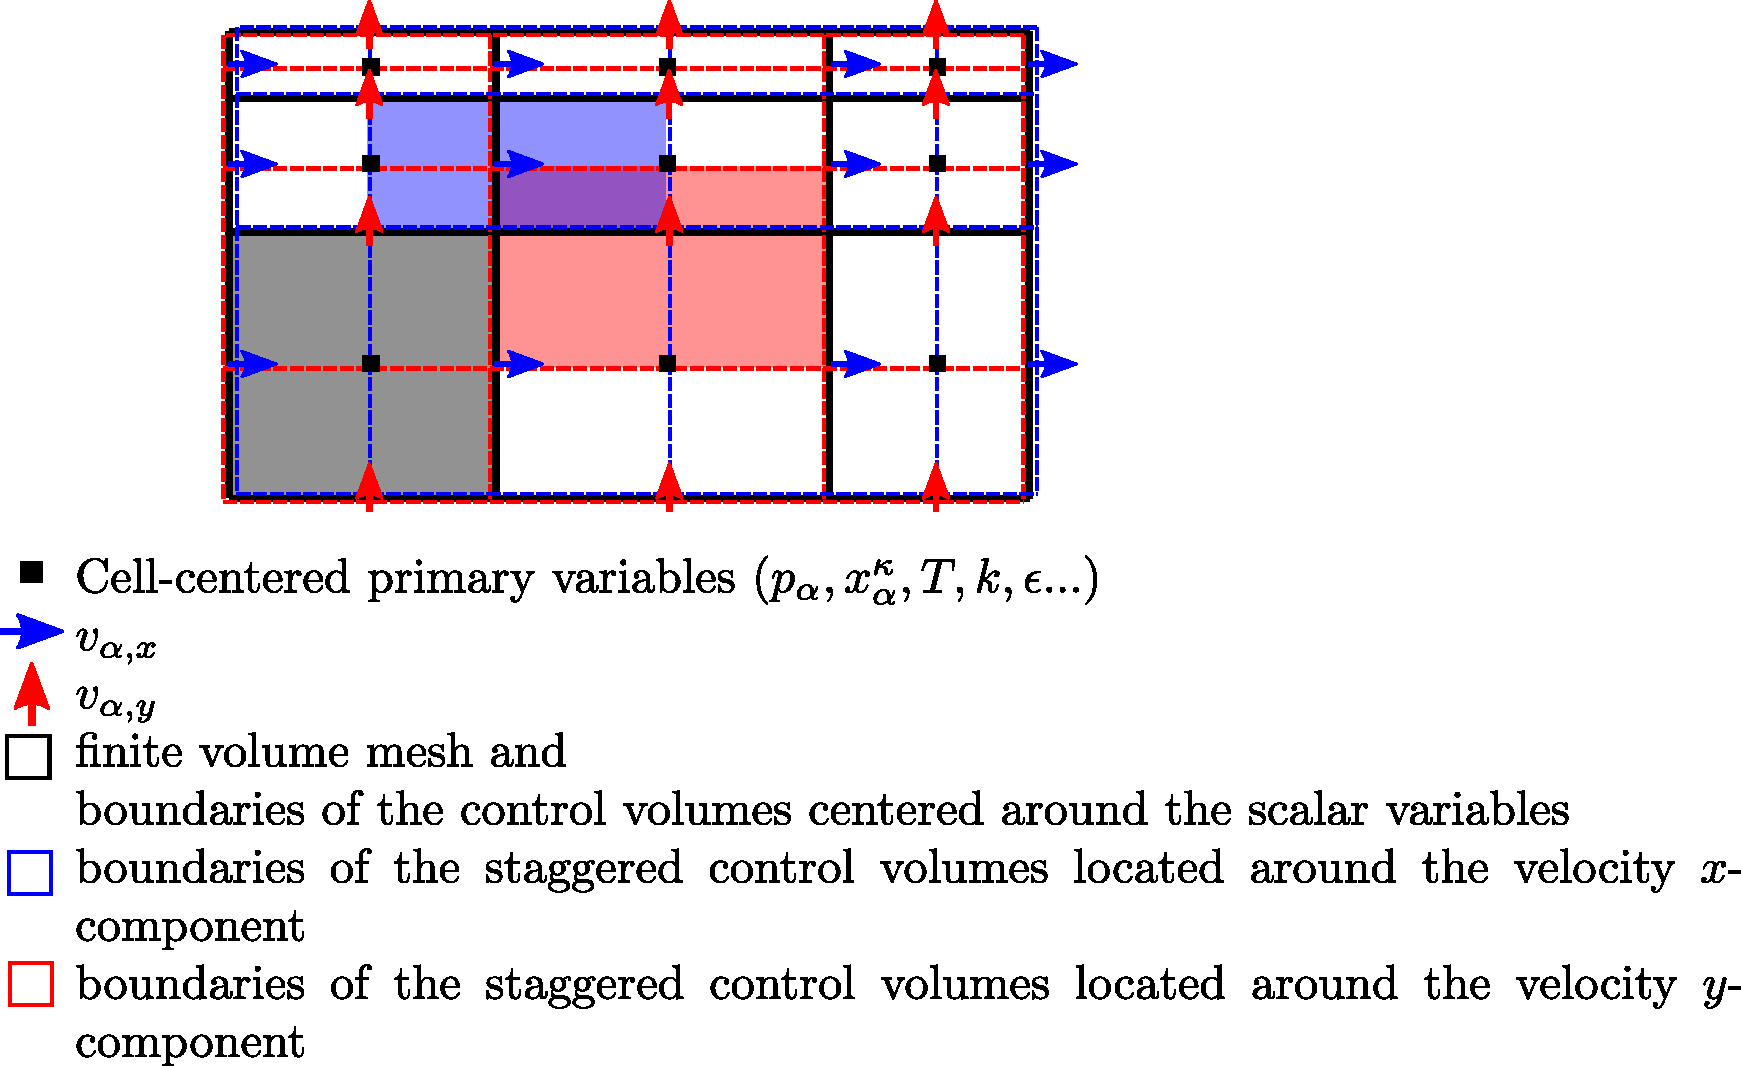
\includegraphics[width=.8\linewidth]{./pdf/staggered_grid.pdf}
\caption{\label{pc:staggered} Discretization of the staggered-grid method. The figure shows the different control volume arrangements, which are staggered with respect to each other. There are the control volumes centered around the scalar primary variables in black, the control volumes located around the $x$-component of the velocity in blue and the control volumes located around the $y$-components of the velocity in red. The control volume boundaries are given by lines. Additionally, there is one shaded example control volume each.\\
In the two-dimensional free-flow models, the continuity equation is discretized using the black control volumes, the $x$-component of the momentum equation is discretized using the blue control volumes and the $y$-component is discretized using the red control volumes. In three dimensions this works analogously.}
\end{figure}

The staggered-grid or marker-and-cell method uses a finite volume method with different control volumes for different equations. There are control volumes centered around the scalar primary variables. They correspond to the finite volume mesh. Additionally, there are control volumes located around the $x,y$ and (in 3D) $z$ velocity components which are shifted in the $x,y$ and $z$ direction, such that the velocity components are located on the edges of the cell-centered finite volume mesh (see Figure~\ref{pc:staggered}). As for the cell-centered method, the fluxes are evaluated at the edges of each control volume with a two-point flux approximation, cf. \ref{cc}.\par
The staggered-grid method is robust, mass conservative, and free of pressure oscillations
but should, as the cell-centered TPFA method, only be applied for structured grids.
Currently, all free-flow models in \Dumux use the staggered-grid discretization.
